\addtocounter{chapter}{0}
\setcounter{figure}{0}
\setcounter{table}{0}
\renewcommand{\thefigure}{7.\arabic{figure}} % يجبر اللاحقة تبدأ برقم 7
\renewcommand{\thetable}{7.\arabic{table}}   % يجبر الجداول تبدأ برقم 7
\section{Introduction}

The continuous advancement of renewable energy technologies, electric vehicles, and power electronic converters has created new opportunities for improving photovoltaic-powered EV charging systems. Although the proposed system demonstrates efficient integration of a photovoltaic array, battery energy storage system, bidirectional AC/DC converter, and electric vehicle charging unit through a common DC link, continuous technological developments offer significant potential for enhancing system efficiency, flexibility, reliability, and overall operational performance.

Future improvements are expected to focus on advanced power conversion technologies, intelligent maximum power point tracking algorithms, energy management strategies, smart charging techniques, and artificial intelligence-based monitoring and control systems. These developments aim to maximize renewable energy utilization, improve power quality, support bidirectional energy flow, and enable more intelligent operation of next-generation photovoltaic-powered EV charging infrastructures.
\section{Advanced Power Conversion Technologies}

Power electronic converters play a vital role in the performance of photovoltaic-powered energy systems. They are responsible for regulating voltage levels, controlling power flow, and ensuring efficient energy conversion between different system components. Continuous developments in converter topologies have led to significant improvements in efficiency, power density, and controllability, making advanced converters an essential component of future renewable energy systems.
\subsection{Dual Active Bridge (DAB) Converter}

The Dual Active Bridge (DAB) converter is a bidirectional isolated DC/DC converter consisting of two active full-bridge converters connected through a high-frequency transformer. The transformer provides galvanic isolation between the input and output ports while enabling efficient power transfer through high-frequency operation. Owing to its symmetrical structure and bidirectional configuration, the DAB converter has become a widely adopted topology in modern high-power DC/DC conversion applications.
\begin{figure}[H]
    \centering
    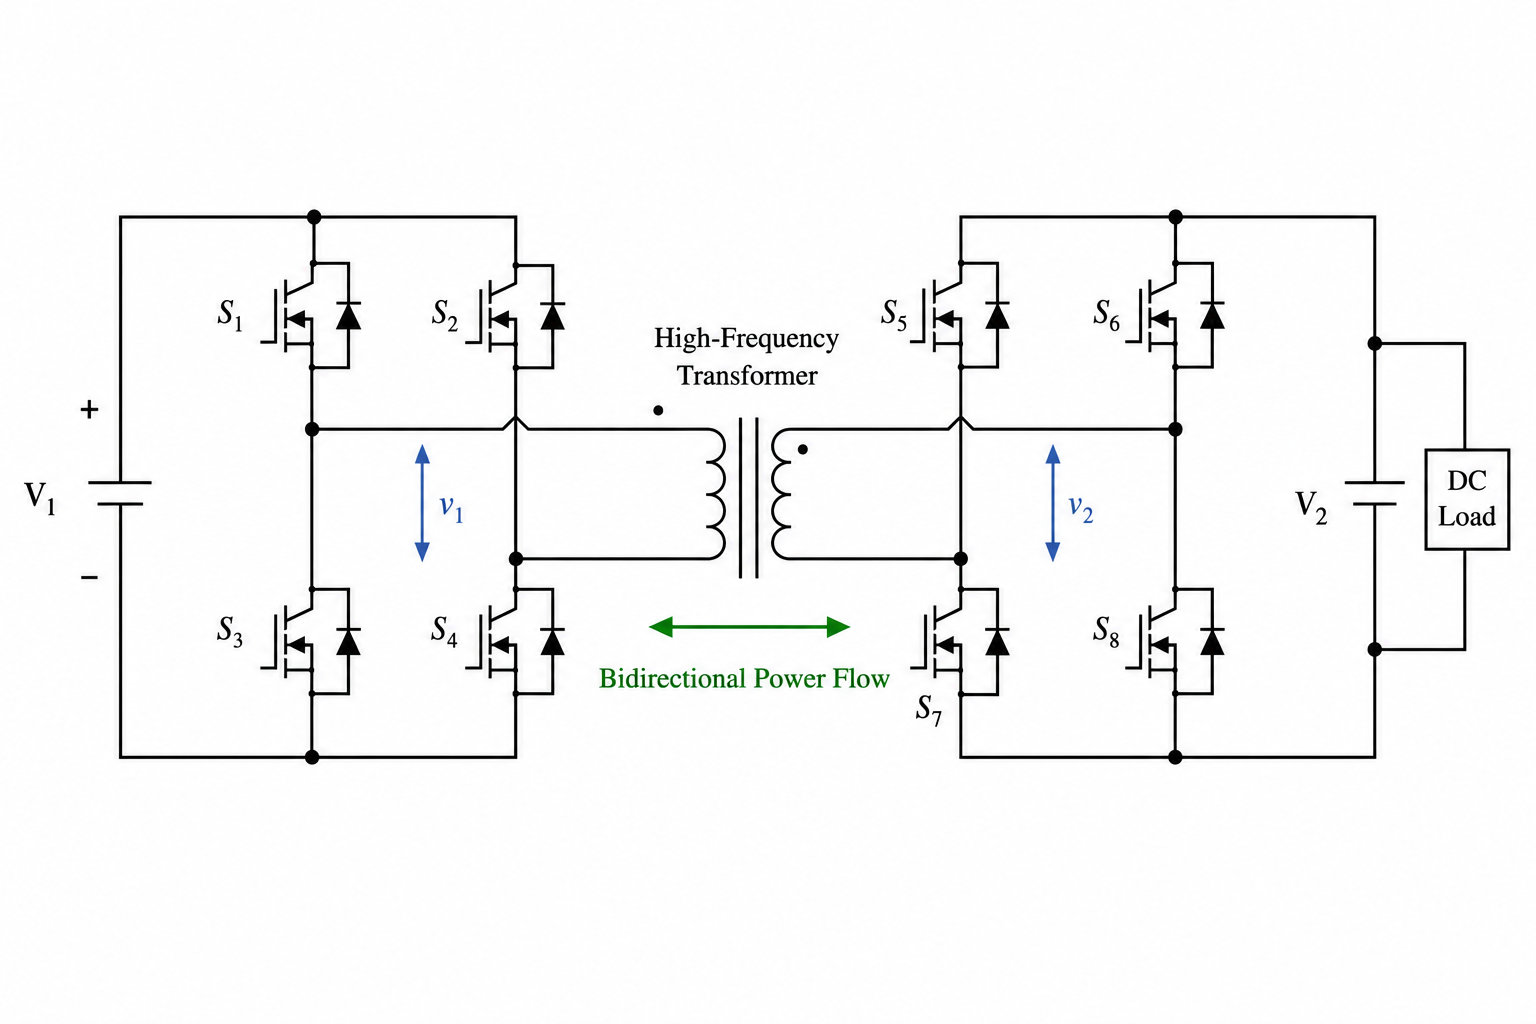
\includegraphics[width=0.8\textwidth]{Figures/Dab.png}
    \caption{Basic structure of the Dual Active Bridge (DAB) converter.}
    \label{fig:dab_converter}
\end{figure}
Power transfer in the DAB converter is achieved by controlling the phase shift between the voltages generated by the primary-side and secondary-side full bridges. The magnitude and direction of the transferred power depend on the phase difference between the two bridges, allowing accurate regulation of power flow. This control method also enables soft-switching operation over a wide operating range, which contributes to reducing switching losses and improving conversion efficiency.
\begin{table}[H]
\caption{Comparison Between Conventional Buck Converter and DAB Converter}
\label{tab:dab_comparison}

\centering
\renewcommand{\arraystretch}{1.5}

\begin{tabularx}{\textwidth}{
>{\raggedright\arraybackslash}p{4cm}
>{\centering\arraybackslash}X
>{\centering\arraybackslash}X
}
\toprule

\textbf{Feature} &
\textbf{Conventional Buck Converter} &
\textbf{Dual Active Bridge (DAB)} \\

\midrule

Power Flow &
Unidirectional &
Bidirectional \\

Galvanic Isolation &
Not Available &
Available \\

Voltage Conversion &
Step-down Only &
Wide Voltage Range \\

Control Method &
PWM Control &
Phase-Shift Control \\

Power Density &
Moderate &
High \\

Soft Switching &
Not Supported &
Supported \\

Application Flexibility &
Limited &
High \\

\bottomrule

\end{tabularx}

\end{table}
\newpage
The combination of bidirectional power transfer, galvanic isolation, soft-switching capability, and flexible phase-shift control makes the DAB converter a highly efficient and reliable DC/DC conversion topology. These technical characteristics allow the converter to operate under a wide range of voltage and power conditions while maintaining high efficiency and compact design. Therefore, the DAB converter is considered a promising candidate for future high-performance power conversion systems.
\subsection{LLC Resonant Converter}
The LLC resonant converter is an isolated DC/DC converter topology that has gained significant attention in high-efficiency power conversion applications. It consists of a resonant tank formed by a resonant inductor, a magnetizing inductor, and a resonant capacitor, together with a high-frequency transformer. This resonant structure enables efficient energy transfer while providing galvanic isolation between the input and output stages.
\begin{figure}[H]
    \centering
    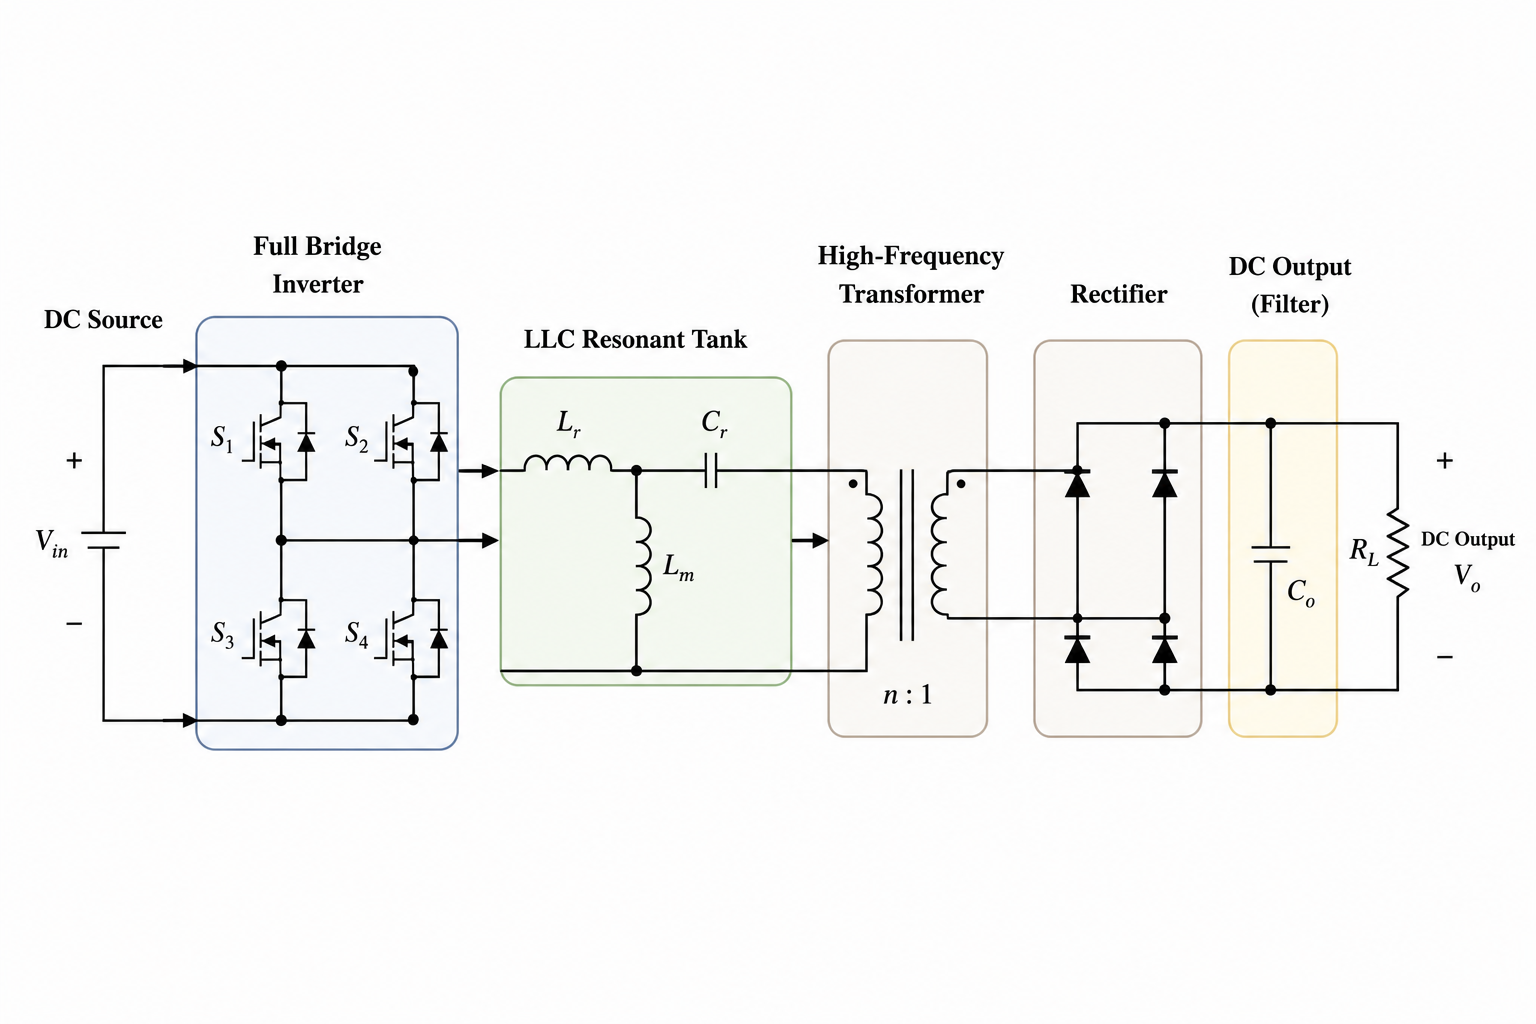
\includegraphics[width=0.85\textwidth]{Figures/LLC.png}
    \caption{Schematic diagram of the LLC resonant converter topology.}
    \label{fig:llc_converter}
\end{figure}

The operating principle of the LLC resonant converter is based on the resonance between the inductive and capacitive elements of the resonant tank. By varying the switching frequency around the resonant frequency, the converter regulates the output voltage while maintaining soft-switching conditions over a wide operating range. This operating mechanism minimizes switching losses and reduces electromagnetic interference, leading to higher conversion efficiency.
\newpage
The LLC resonant converter combines high conversion efficiency, soft-switching capability, and compact converter design within a single topology. Its ability to achieve Zero Voltage Switching (ZVS) under most operating conditions significantly improves converter efficiency while reducing thermal stress on switching devices. These characteristics make the LLC resonant converter a promising solution for future high-performance isolated DC/DC power conversion systems.
The continuous development of advanced converter topologies provides a solid foundation for improving the overall efficiency of photovoltaic-powered energy systems. However, maximizing the harvested solar energy also requires intelligent control strategies capable of continuously tracking the maximum available power under varying environmental conditions. Therefore, advanced Maximum Power Point Tracking (MPPT) techniques have become an important area of future research and development.
\subsection{Wide-Bandgap Semiconductor Devices}
Wide-bandgap (WBG) semiconductor devices represent a significant advancement in modern power electronics. Unlike conventional silicon (Si) devices, WBG semiconductors possess a considerably larger energy bandgap, enabling operation under higher electric fields, higher switching frequencies, and elevated junction temperatures. These characteristics make WBG devices highly suitable for next-generation power converters used in renewable energy systems and electric vehicle charging infrastructures\cite{baliga2008}.
The superior performance of WBG semiconductor devices is mainly attributed to their wider energy bandgap. Conventional silicon has a bandgap energy of approximately 1.12 eV, whereas Silicon Carbide (SiC) and Gallium Nitride (GaN) possess significantly larger bandgap energies of approximately 3.26 eV and 3.40 eV, respectively. The wider bandgap increases the critical electric field, reduces leakage current, and allows operation at higher junction temperatures with lower switching losses. Consequently, converters based on WBG devices can achieve higher efficiency, higher power density, and improved thermal performance compared with conventional silicon-based converters\cite{baliga2008,wolfspeed}.
\begin{figure}[H]
    \centering
    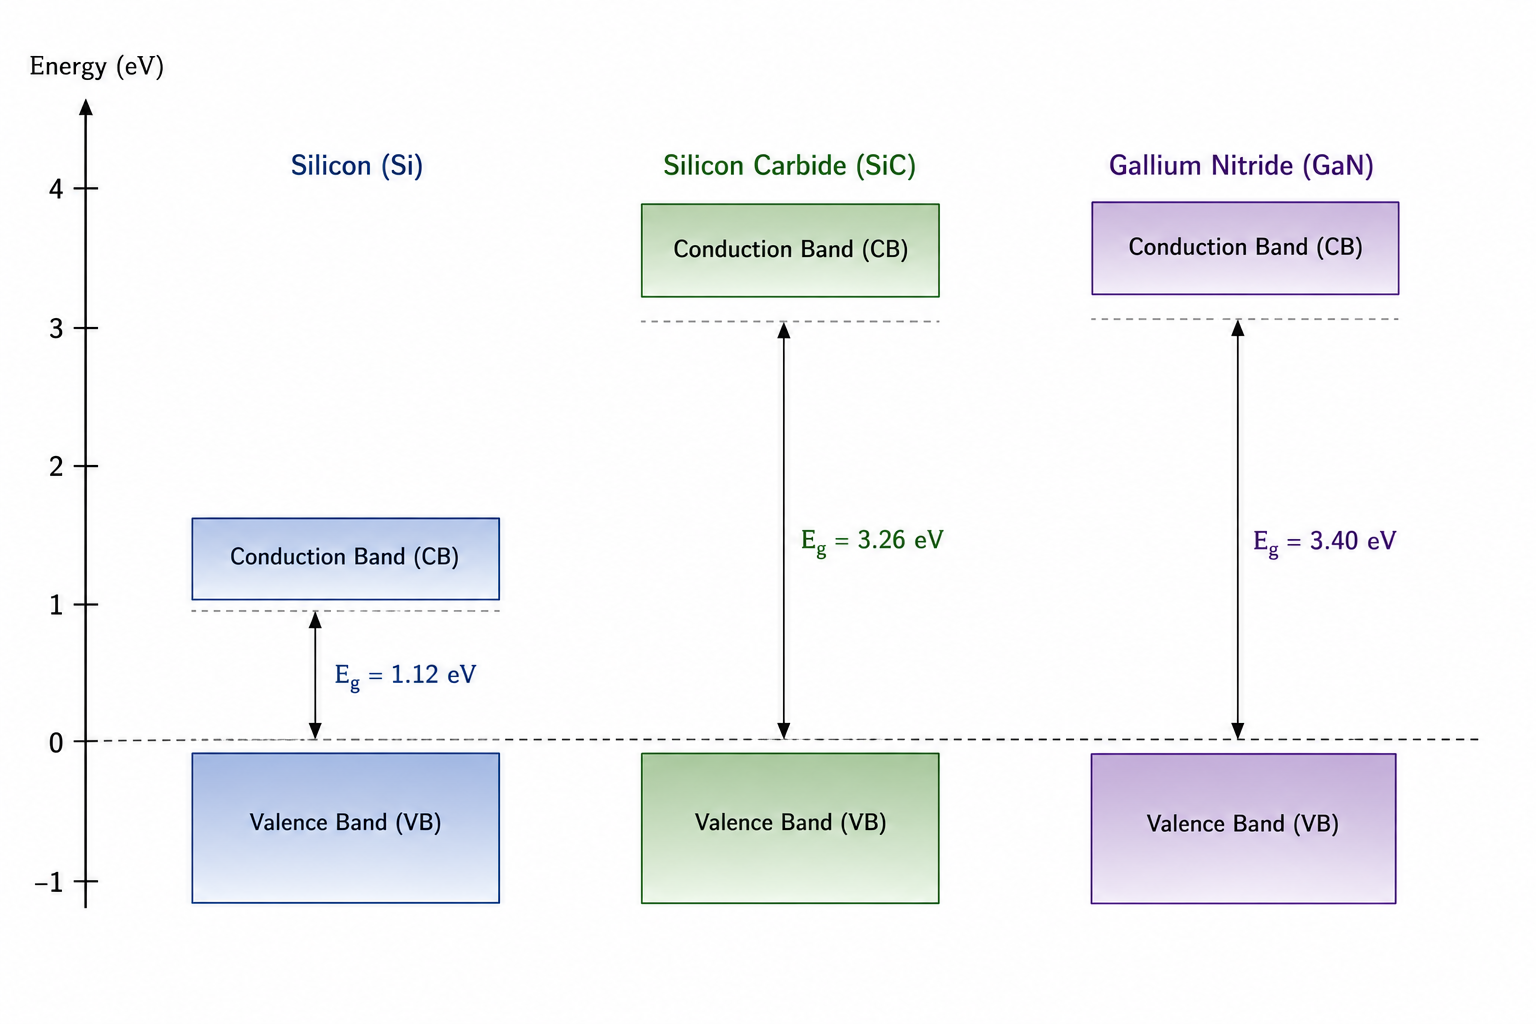
\includegraphics[width=0.85\textwidth]{Figures/WBG.png}
    \caption{Energy bandgap comparison between Silicon (Si), Silicon Carbide (SiC), and Gallium Nitride (GaN).}
    \label{fig:wbg_bandgap}
\end{figure}
Silicon Carbide (SiC) is widely adopted in medium- and high-power electronic converters due to its high breakdown electric field, excellent thermal conductivity, and high-temperature capability. These properties enable SiC devices to operate at higher voltages while reducing conduction and switching losses. As a result, SiC technology is particularly suitable for high-power renewable energy systems, grid-connected converters, and battery energy storage applications\cite{wolfspeed}.
Gallium Nitride (GaN) is characterized by extremely high electron mobility and low parasitic capacitance, allowing significantly faster switching speeds than conventional silicon devices. These characteristics enable high-frequency converter operation with reduced switching losses and smaller passive components, resulting in compact converter designs with high power density. Therefore, GaN devices are considered an attractive solution for future high-frequency power electronic applications\cite{baliga2008}.
\begin{table}[H]
\caption{Comparison of Semiconductor Material Properties}
\label{tab:wbg_properties}

\centering
\renewcommand{\arraystretch}{1.4}

\begin{tabularx}{\textwidth}{
>{\raggedright\arraybackslash}p{4.8cm}
>{\centering\arraybackslash}X
>{\centering\arraybackslash}X
>{\centering\arraybackslash}X
}
\toprule

\textbf{Property} &
\textbf{Silicon (Si)} &
\textbf{Silicon Carbide (SiC)} &
\textbf{Gallium Nitride (GaN)} \\

\midrule

Bandgap Energy (eV) &
1.12 &
3.26 &
3.40 \\

Critical Electric Field (MV/cm) &
0.3 &
3.0 &
3.3 \\

Thermal Conductivity (W/cm·K) &
1.5 &
4.9 &
1.3 \\

Maximum Junction Temperature (°C) &
150 &
200--250 &
200 \\

Switching Frequency &
Moderate &
High &
Very High \\

Switching Losses &
High &
Low &
Very Low \\

\bottomrule

\end{tabularx}

\end{table}
The continuous development of WBG semiconductor devices is expected to accelerate the transition toward highly efficient and compact power electronic converters. Their superior electrical characteristics enable higher switching frequencies, lower power losses, and improved thermal performance, making SiC- and GaN-based devices promising candidates for next-generation photovoltaic-powered EV charging systems.

\section{Advanced MPPT Techniques}
Maximum Power Point Tracking (MPPT) remains one of the most active research areas in photovoltaic energy systems. As photovoltaic-powered electric vehicle charging stations become increasingly intelligent and interconnected, future MPPT techniques are expected to move beyond conventional optimization methods toward adaptive, data-driven, and self-learning approaches. Recent advances in artificial intelligence, computational intelligence, and optimization algorithms have enabled the development of MPPT techniques capable of improving tracking accuracy, reducing convergence time, and maintaining high energy extraction efficiency under rapidly changing environmental conditions.
\subsection{Artificial Intelligence-Based MPPT}
Artificial intelligence (AI) has emerged as one of the most promising technologies for future MPPT applications in photovoltaic systems. By utilizing data-driven learning algorithms, AI-based controllers can analyze complex relationships between environmental conditions and photovoltaic output characteristics without relying on predefined mathematical models. This capability enables rapid identification of the maximum power point while reducing steady-state oscillations and improving tracking performance under rapidly changing irradiance and temperature conditions.
\begin{figure}[!htbp]
    \centering
    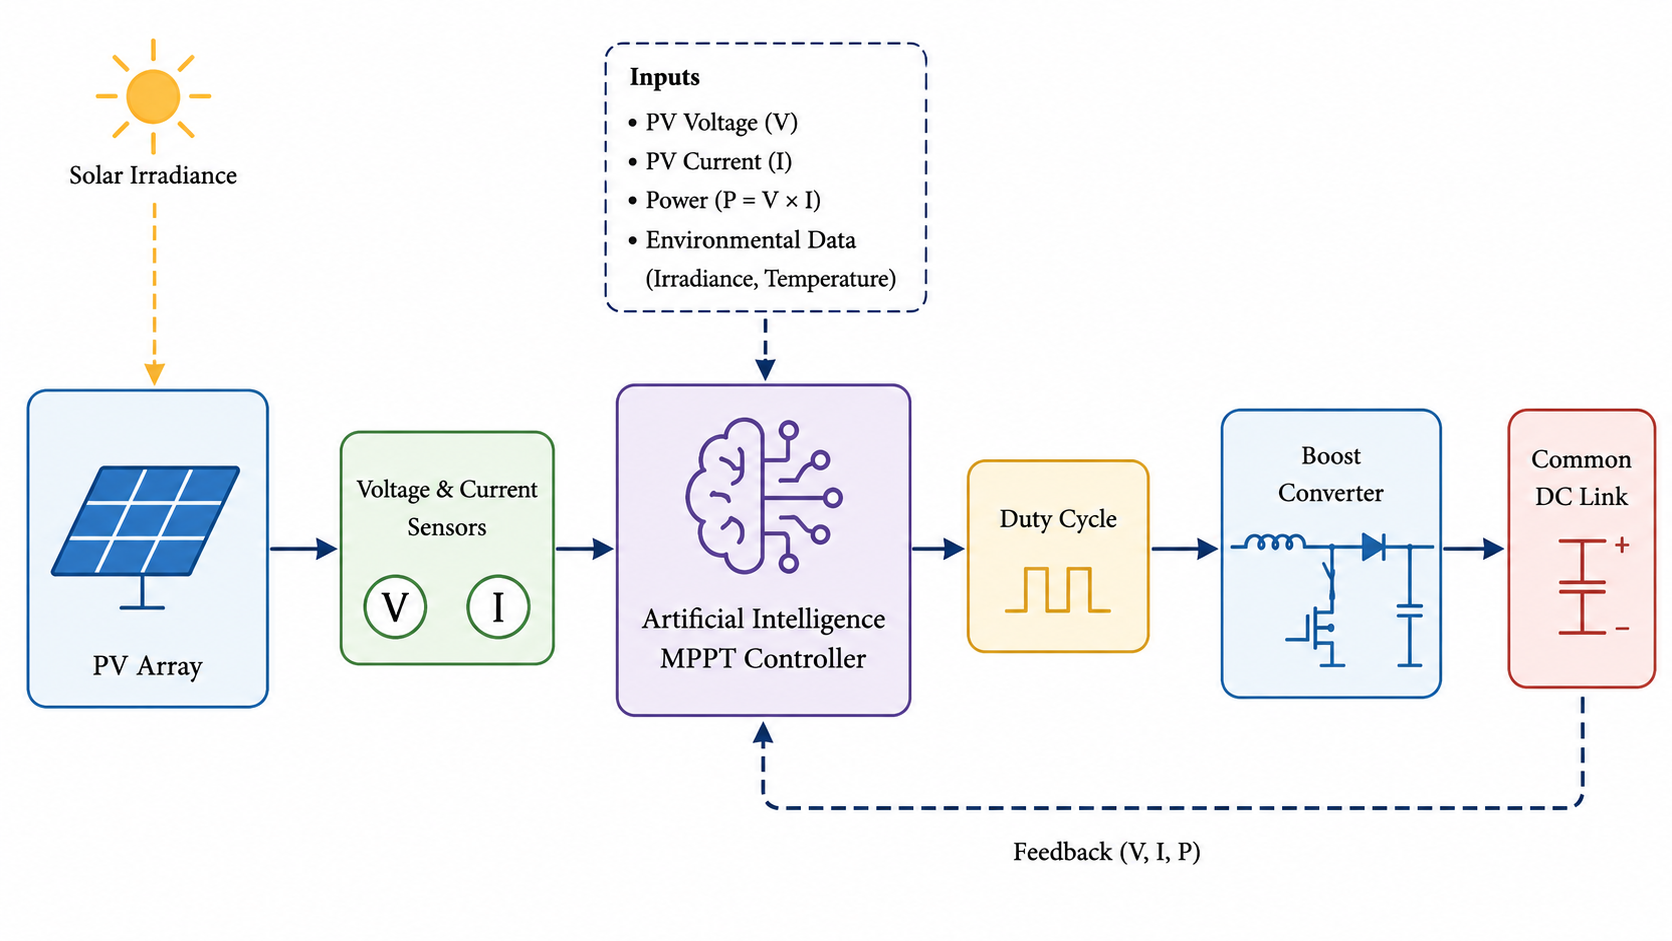
\includegraphics[width=0.85\textwidth]{Figures/mppt AI.png}
    \caption{Conceptual architecture of an artificial intelligence-based MPPT system for future photovoltaic applications.}
    \label{fig:ai_mppt}
\end{figure}
\subsection{Fuzzy Logic MPPT}

Fuzzy Logic Control (FLC) has become one of the most widely investigated intelligent MPPT techniques due to its ability to handle nonlinear and uncertain operating conditions without requiring an accurate mathematical model of the photovoltaic system. Instead of relying on fixed equations, fuzzy logic utilizes linguistic rules and membership functions to determine the appropriate control action based on variations in photovoltaic voltage and power. This approach enables rapid tracking of the maximum power point while maintaining stable operation during sudden variations in solar irradiance and temperature.

Despite these advantages, the performance of fuzzy logic-based MPPT depends significantly on the proper design of membership functions and fuzzy inference rules. Developing an effective rule base often requires expert knowledge and may become increasingly complex as the operating conditions of the photovoltaic system become more diverse. Nevertheless, its robustness and fast dynamic response make fuzzy logic a promising candidate for future photovoltaic-powered EV charging systems.
\subsection{Artificial Neural Network-Based MPPT}

Artificial Neural Networks (ANNs) have emerged as powerful data-driven techniques for maximum power point tracking due to their ability to learn complex nonlinear relationships between environmental variables and photovoltaic system characteristics. By utilizing historical operating data during the training process, an ANN can accurately estimate the operating point corresponding to the maximum available power under different irradiance and temperature conditions. This capability significantly improves tracking speed, minimizes steady-state oscillations, and enhances the overall energy conversion efficiency of photovoltaic systems.
\newpage
However, the effectiveness of ANN-based MPPT strongly depends on the quality and quantity of the training dataset. The training process may require considerable computational resources and time before achieving reliable prediction accuracy. Furthermore, network retraining may be necessary when the photovoltaic system operates under conditions that differ significantly from the original training data. Despite these challenges, advances in embedded computing and artificial intelligence continue to improve the practicality of ANN-based MPPT for future intelligent charging infrastructures.
\subsection{Reinforcement Learning-Based MPPT}

Reinforcement Learning (RL) has recently emerged as an advanced artificial intelligence technique for maximum power point tracking in photovoltaic systems. Unlike supervised learning approaches, reinforcement learning continuously interacts with the operating environment and improves its control strategy through trial-and-error learning. By receiving feedback in the form of rewards, the controller gradually learns the optimal control policy capable of maximizing photovoltaic power generation under varying environmental conditions.

Although reinforcement learning offers excellent adaptability and self-learning capabilities, its implementation remains computationally demanding. The controller generally requires extensive training before achieving stable performance, and convergence may be relatively slow during the learning phase. In addition, designing an appropriate reward function is essential for ensuring reliable operation. Nevertheless, continuous developments in artificial intelligence and high-performance embedded processors are expected to facilitate the practical implementation of RL-based MPPT in next-generation photovoltaic-powered EV charging stations.
\begin{table}[H]
\caption{Comparison of Intelligent MPPT Techniques for Future Photovoltaic Systems}
\label{tab:mppt_comparison}

\centering
\renewcommand{\arraystretch}{1.5}

\begin{tabularx}{\textwidth}{
>{\raggedright\arraybackslash}p{4.6cm}
>{\centering\arraybackslash}p{2cm}
>{\centering\arraybackslash}p{2.2cm}
>{\centering\arraybackslash}X
}
\toprule

\textbf{MPPT Technique} &
\textbf{Accuracy} &
\textbf{Tracking Speed} &
\textbf{Complexity} \\

\midrule

Fuzzy Logic &
High &
Fast &
Medium \\

Artificial Neural Network (ANN) &
Very High &
Fast &
High \\

Reinforcement Learning (RL) &
Very High &
Adaptive &
High \\

\bottomrule

\end{tabularx}

\end{table}
The continuous development of intelligent MPPT algorithms is expected to further improve the efficiency of photovoltaic energy harvesting under complex environmental conditions. However, maximizing the generated energy alone is not sufficient to achieve optimal overall system performance. Future photovoltaic-powered EV charging systems also require intelligent strategies capable of efficiently managing the generated, stored, and consumed energy. Therefore, advanced Energy Management Systems (EMS) are expected to become an essential component of future charging infrastructures.
\section{Energy Management System (EMS)}

An Energy Management System (EMS) is a supervisory control system responsible for coordinating the operation of all power sources and loads within the charging station. Rather than performing power conversion directly, the EMS continuously collects operating data, processes system information, and determines the appropriate operating mode according to predefined control objectives\cite{tie2013}.
The EMS consists of measurement units, a central controller, communication interfaces, and an optimization algorithm. The measurement units acquire real-time information such as photovoltaic output power, battery state of charge, charging demand, DC-link voltage, and grid status. These measurements are transmitted to the controller, where they are analyzed before appropriate control commands are generated for the different power electronic converters.
\begin{figure}[H]
    \centering
    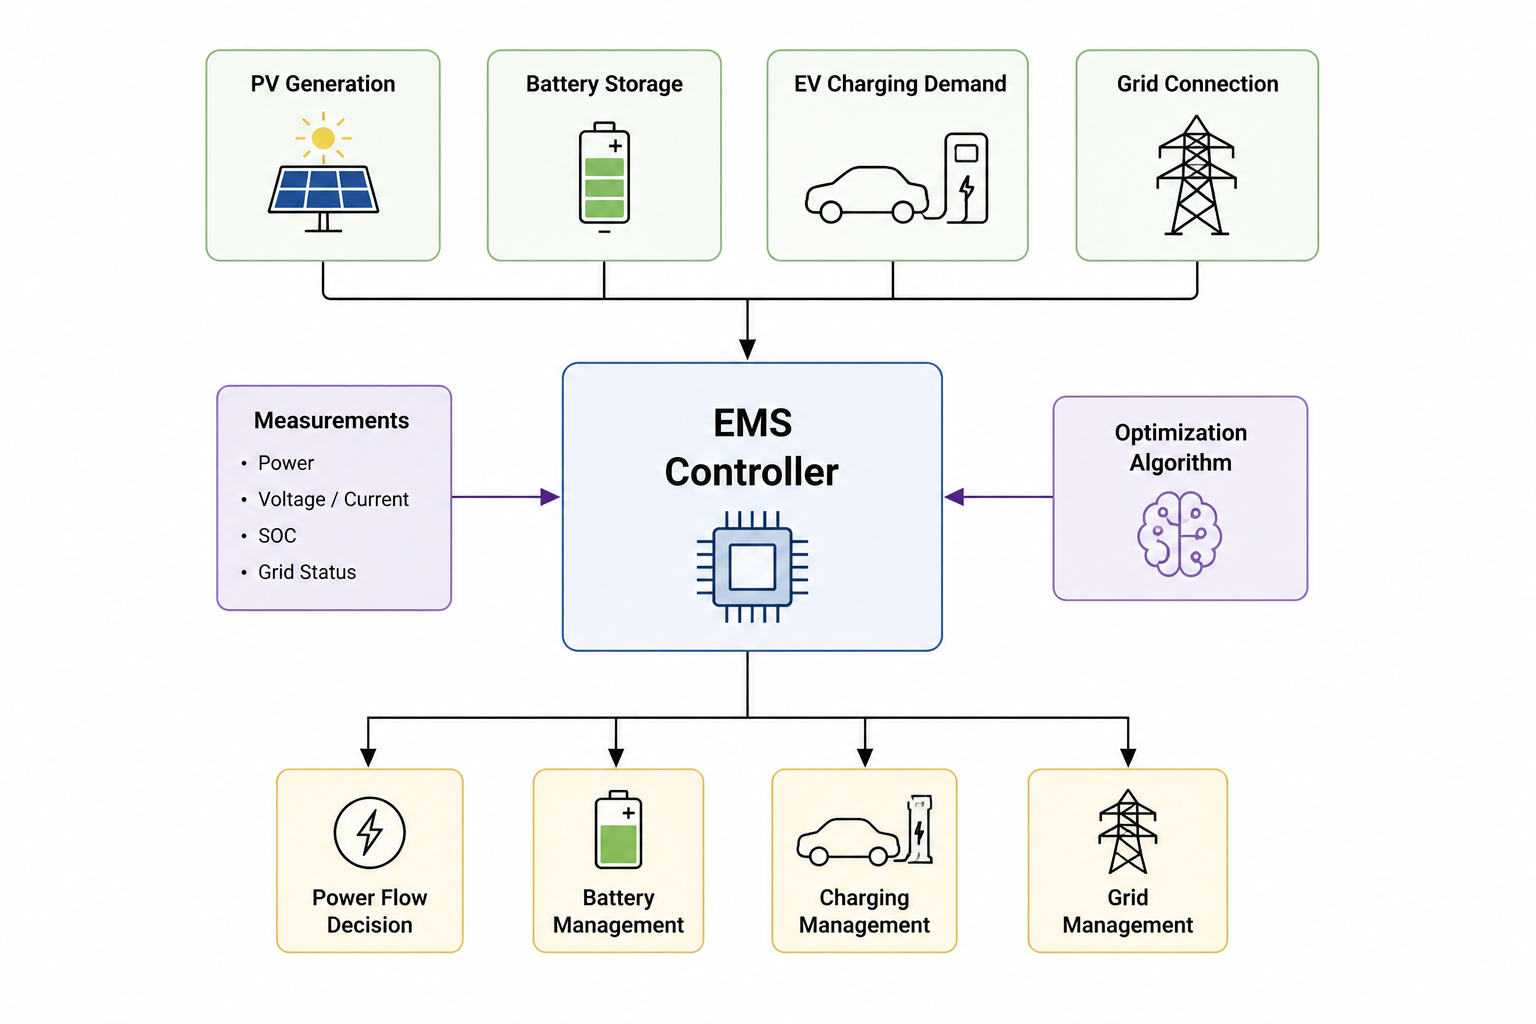
\includegraphics[width=0.85\textwidth]{Figures/EMS.png}
    \caption{Architecture of the Energy Management System (EMS).}
    \label{fig:ems_architecture}
\end{figure}
The operating principle of the EMS is based on continuous monitoring, decision-making, and control. During operation, the controller periodically receives measurements from all system components and evaluates the current operating conditions. Based on the selected optimization strategy, the EMS determines the required operating mode and generates control signals for the corresponding power converters to regulate energy flow throughout the system.
\newpage
\section{Smart Charging Technologies}
Smart charging is an advanced charging strategy that dynamically regulates the charging process of electric vehicles according to the operating conditions of the charging station. Unlike conventional charging, which delivers constant charging power regardless of system conditions, smart charging continuously adjusts the charging power based on the available photovoltaic generation, battery energy storage status, grid conditions, and charging demand. This coordinated control enables more efficient utilization of available energy resources while maintaining reliable system operation\cite{tie2013,emadi2015}.
The operating principle of smart charging relies on continuous communication between the Energy Management System (EMS) and the charging controller. During operation, the EMS monitors the available photovoltaic power, battery state of charge, charging demand, and grid conditions. Based on these measurements, the controller determines the appropriate charging power and charging schedule before transmitting control commands to the EV charger. Consequently, the charging process continuously adapts to changing operating conditions while maintaining stable system performance.
\begin{figure}[H]
    \centering
    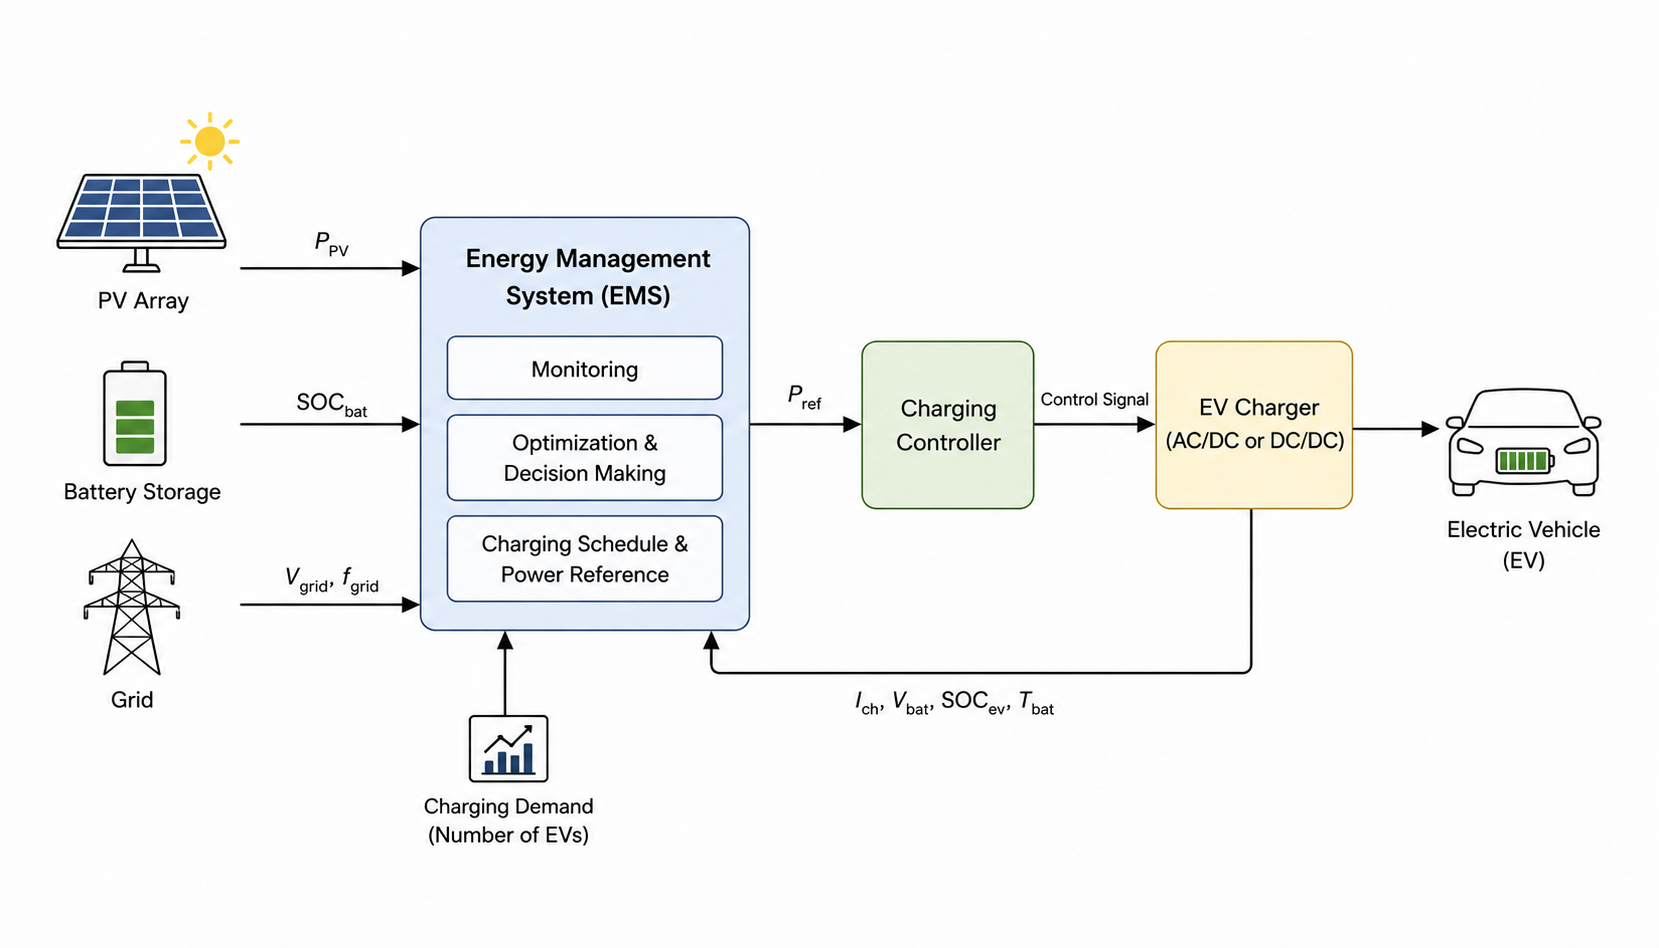
\includegraphics[width=\textwidth]{Figures/smart charge.png}
    \caption{Architecture of a smart EV charging system.}
    \label{fig:smart_charging_architecture}
\end{figure}
\subsection{Charging Strategies}
Three charging strategies are commonly employed in smart EV charging systems: uncontrolled charging, scheduled charging, and dynamic smart charging. Their operating principles and characteristics are summarized in Table~\ref{tab:charging_strategies}.
\begin{table}[H]
\caption{Comparison of Smart Charging Strategies}
\label{tab:charging_strategies}

\centering
\renewcommand{\arraystretch}{1.4}

\begin{tabularx}{\textwidth}{
>{\raggedright\arraybackslash}p{3.8cm}
>{\raggedright\arraybackslash}X
>{\raggedright\arraybackslash}X
}
\toprule

\textbf{Charging Strategy} &
\textbf{Operating Principle} &
\textbf{Typical Characteristics} \\

\midrule

Uncontrolled Charging &
The EV begins charging immediately after connection. &
Simple implementation but may increase peak demand and grid loading. \\

Scheduled Charging &
Charging is performed during predefined time intervals according to user preferences or electricity tariffs. &
Reduces charging cost and improves load distribution. \\

Dynamic Smart Charging &
Charging power is continuously adjusted according to PV generation, battery SOC, charging demand, and grid conditions. &
Provides optimal energy utilization, improved grid support, and enhanced operational flexibility. \\

\bottomrule

\end{tabularx}

\end{table}
Among these strategies, dynamic smart charging has attracted significant research interest due to its ability to continuously adapt the charging process to changing operating conditions. By coordinating photovoltaic generation, battery energy storage, and grid interaction through the EMS, the charging controller can determine the optimal charging power in real time. This adaptive operation improves renewable energy utilization, reduces unnecessary grid power consumption, and enhances the overall performance of photovoltaic-powered EV charging stations.
\section{Vehicle-to-Grid (V2G)}
Vehicle-to-Grid (V2G) is a bidirectional energy exchange technology that enables electric vehicles to operate as distributed energy storage units in addition to their primary transportation function. During V2G operation, the energy stored in the EV battery can be supplied back to the power system whenever additional electrical support is required. This bidirectional capability enhances the flexibility of future photovoltaic-powered charging infrastructures and contributes to more efficient energy utilization.
The operating principle of V2G is based on bidirectional power transfer between the electric vehicle battery and the common DC link of the charging station. During normal charging, electrical energy flows from the photovoltaic system, battery energy storage system, or utility grid to the EV battery through the bidirectional DC/DC converter. When V2G operation is activated, the direction of power flow is reversed, allowing the stored energy to be transferred from the EV battery to the common DC link. The grid-connected bidirectional inverter subsequently converts the DC power into synchronized AC power before injecting it into the utility grid under the supervision of the Energy Management System (EMS).
\begin{figure}[H]
    \centering
    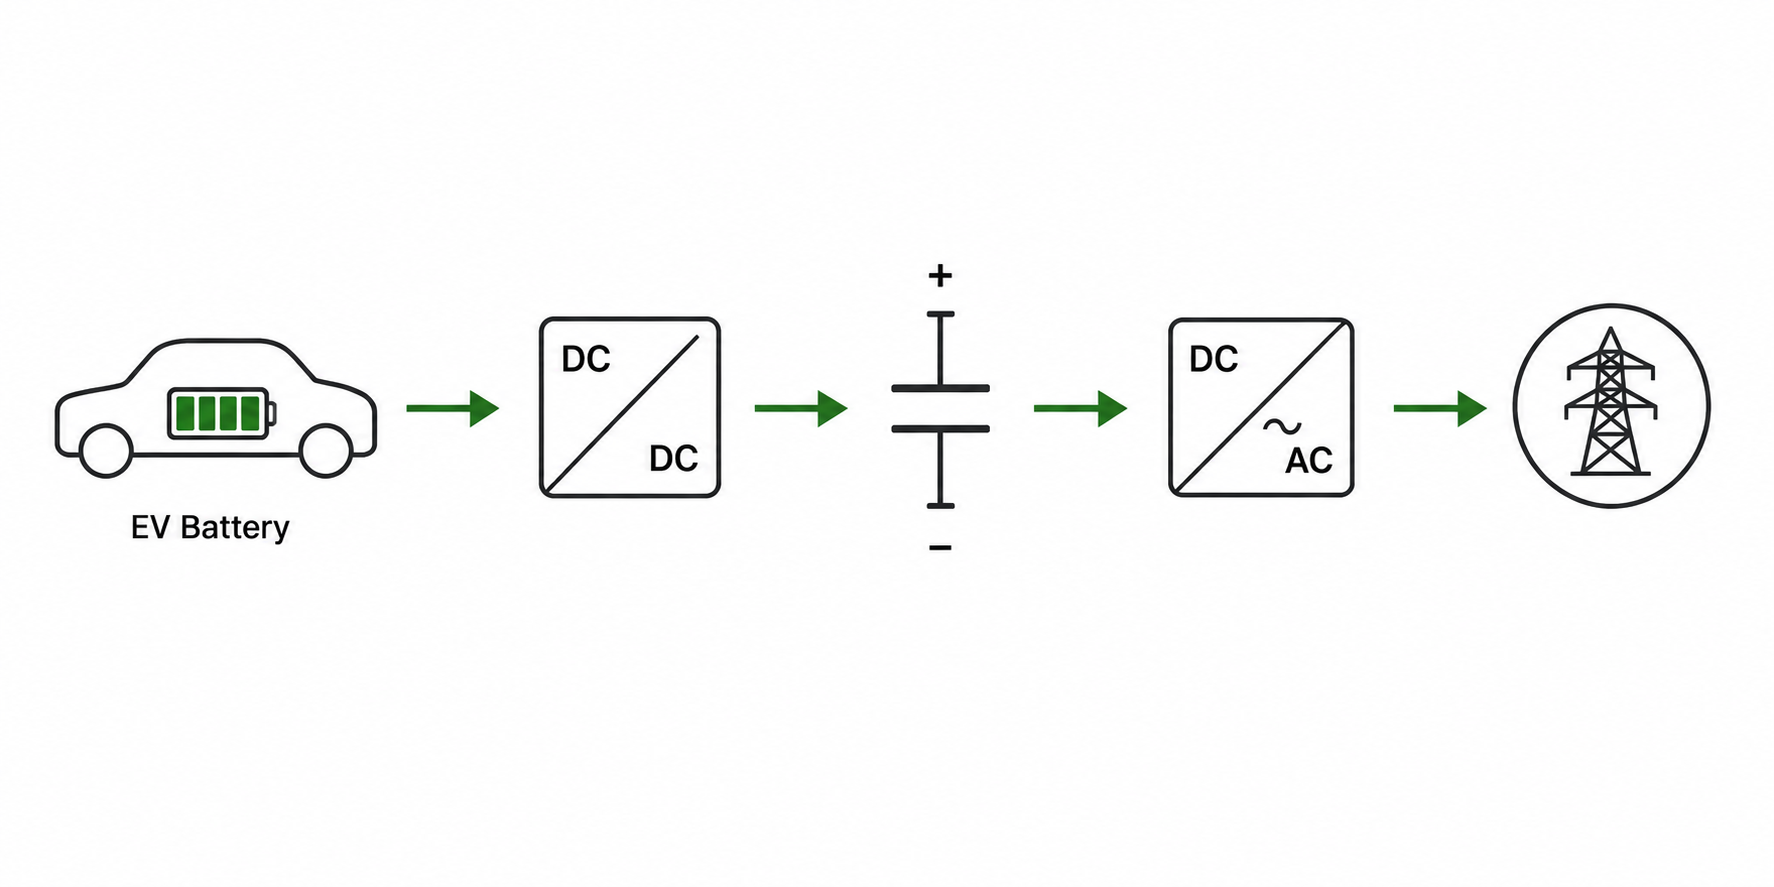
\includegraphics[width=0.9\textwidth]{Figures/V2G.png}
    \caption{Power flow path during Vehicle-to-Grid (V2G) operation.}
    \label{fig:v2g_operation_path}
\end{figure}
The implementation of V2G transforms electric vehicles into active energy resources that can support both the charging station and the utility grid. By coordinating bidirectional energy transfer through the EMS, surplus energy stored in EV batteries can be utilized during periods of high demand or limited photovoltaic generation. Future research is expected to focus on intelligent power scheduling, battery degradation mitigation, and standardized communication protocols to improve the reliability and large-scale deployment of V2G technology.
\section{Artificial Intelligence and IoT Integration}
Artificial Intelligence (AI) and the Internet of Things (IoT) are expected to play an essential role in the next generation of photovoltaic-powered EV charging stations. IoT enables continuous acquisition of real-time data from different system components, while AI utilizes these data to improve operational decision-making through prediction, optimization, and intelligent control. The integration of both technologies enhances the adaptability and efficiency of future charging infrastructures\cite{rehmani2018}.
In an AI-enabled charging station, sensors continuously collect operating data from the photovoltaic system, battery energy storage system, utility grid, and EV charger. These measurements are transmitted through IoT communication networks to a central controller or cloud platform, where AI algorithms analyze the system status and predict future operating conditions. The resulting decisions are then communicated to the Energy Management System (EMS), which generates appropriate control commands for the power converters and charging controller.
\begin{figure}[H]
    \centering
    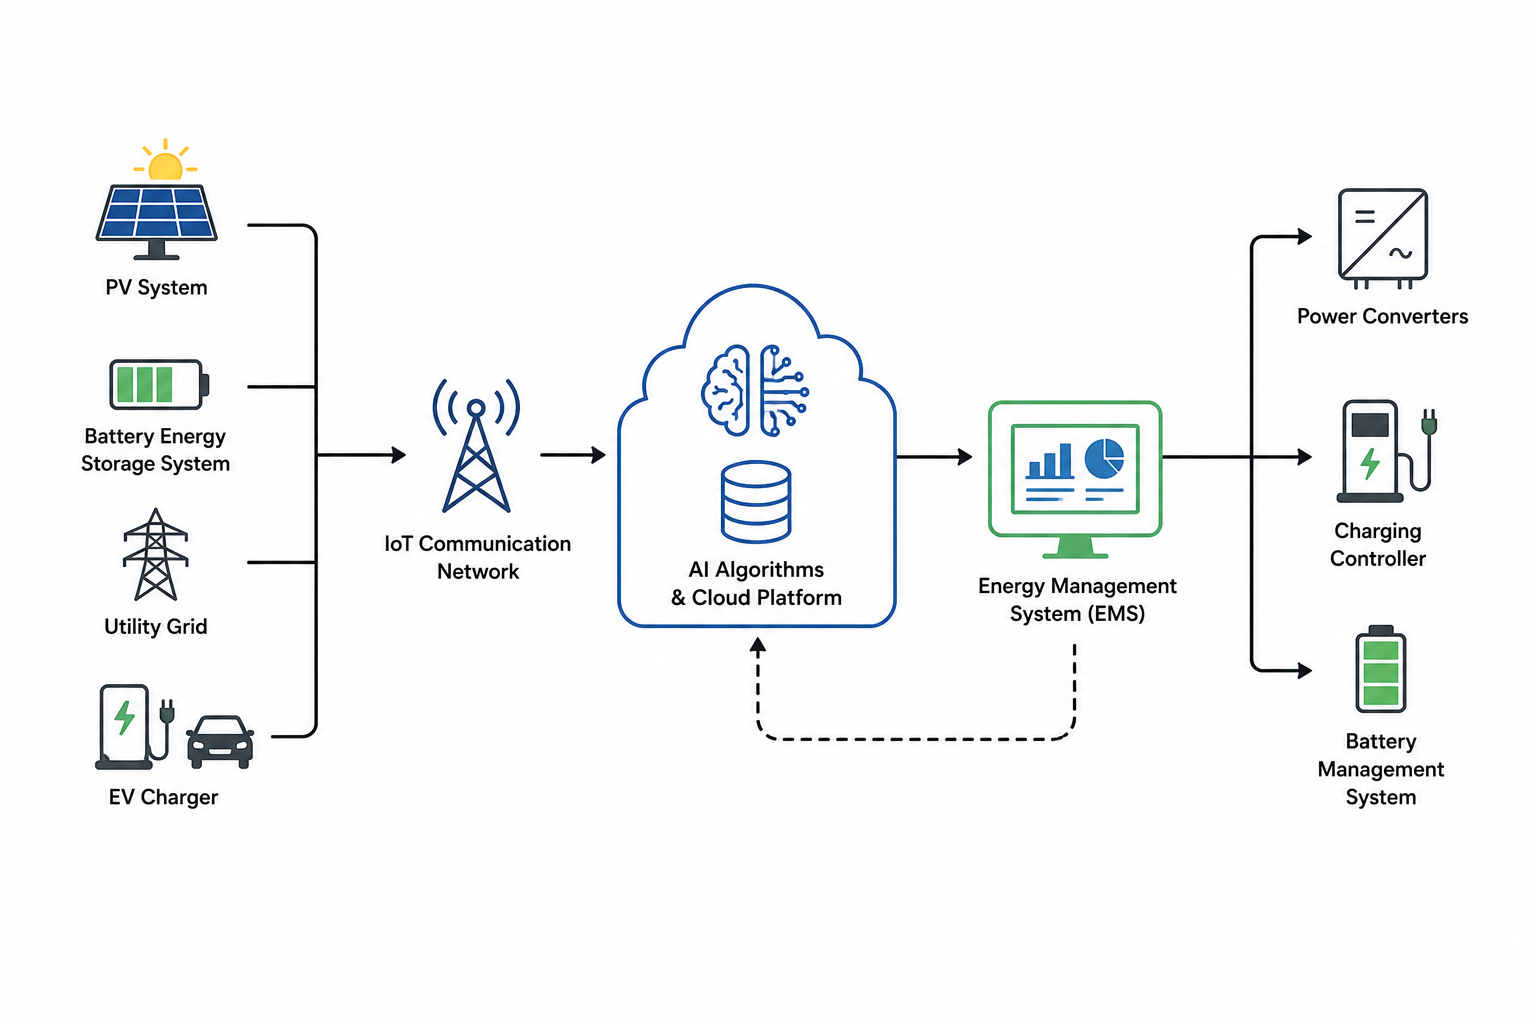
\includegraphics[width=\textwidth]{Figures/AI.png}
    \caption{AI and IoT integration framework for future photovoltaic-powered EV charging stations.}
    \label{fig:ai_iot_integration}
\end{figure}
The integration of AI and IoT enables predictive energy management, adaptive charging strategies, and real-time system optimization. Machine learning algorithms can forecast photovoltaic generation, charging demand, and battery state of charge, allowing the EMS to proactively optimize power allocation. Furthermore, cloud-based monitoring facilitates remote supervision, predictive maintenance, and continuous performance analysis, improving the reliability and operational efficiency of future smart charging stations\cite{rehmani2018}.
\section{Chapter Summary}
This chapter presented several promising future improvements for photovoltaic-powered EV charging stations. Advanced bidirectional DC/DC converters, such as the Dual Active Bridge (DAB), offer enhanced power transfer capability, galvanic isolation, and greater operational flexibility. Intelligent Energy Management Systems (EMS) enable optimal coordination between photovoltaic generation, battery energy storage, electric vehicle charging, and the utility grid. Furthermore, smart charging technologies and Vehicle-to-Grid (V2G) operation improve energy utilization while increasing grid support capabilities. Finally, the integration of Artificial Intelligence (AI), the Internet of Things (IoT), and wide-bandgap semiconductor devices is expected to further enhance the efficiency, reliability, and intelligence of future charging infrastructures. These technological advancements represent important research directions for the development of next-generation renewable energy-based EV charging systems.
